% pdf/a 
\begin{filecontents*}[overwrite]{\jobname.xmpdata}
    \Title{}
    \Author{Gekkó csapat: Bak Bálint, Kozma Dávid Márk, Szilágyi Gábor}
    \Language{hu-HU}
    \Subject{Elektromágneses Terek házi feladat: Föld alatti fémkeresés örvényáramú vizsgálattal}
    \Keywords{EM szimuláció, végeselem, MATLAB, pdetool, házi feladat}
    \Publisher{Gekkó csapat}
\end{filecontents*}

\documentclass[a4paper,12pt,oneside]{article}
\usepackage{ucs}
\usepackage[T1]{fontenc}
\usepackage[utf8]{inputenc}
\usepackage[magyar]{babel}
\usepackage{amsfonts}
\usepackage{amsmath,bm}
\usepackage{pdfpages}
\usepackage{amssymb}
\usepackage{graphicx}
\usepackage[hang]{caption}
\usepackage{lipsum}
\usepackage{wrapfig}
%\usepackage{subcaption}
%\usepackage{enumerate}
%\usepackage{psfrag}
\usepackage[left=10mm,right=10mm,top=10mm,bottom=10mm]{geometry}
\usepackage{hyperref}
%\usepackage{listings}
%\usepackage{cite}
%\usepackage{csquotes}
\usepackage[range-phrase=--, range-units=single]{siunitx}
\usepackage{xcolor}
\usepackage[a-3u]{pdfx}
\hypersetup{
    colorlinks,
%    linkcolor={red!50!black},
    linkcolor={black},
%    citecolor={blue!50!black},
    citecolor={black},
%    urlcolor={blue!80!black}
    urlcolor={blue!80!black}
}

\sloppy % Margón túllógó sorok tiltása.
\widowpenalty=10000 \clubpenalty=10000 %A fattyú- és árvasorok elkerülése
\def\hyph{-\penalty0\hskip0pt\relax} % Kötőjeles szavak elválasztásának engedélyezése

\graphicspath{{kep/}} % ebben a könyvtárban keres képet
\frenchspacing

%\sisetup{per-mode=power}

\DeclareMathOperator{\rot}{rot}
\DeclareMathOperator{\divergence}{div}

\pagestyle{plain} 
\pagenumbering{gobble}
\nopagebreak

\title{
    \centering
    \vspace{-0.8cm}
    
\includegraphics[width=0.3\textwidth]{bme_logo.pdf} \\
    \textbf{Elektromágneses Terek (VIHVMA08)\\
    csoportos házi feladat} \\[2ex]
    Föld alatti fémkeresés örvényáramú vizsgálattal
    \vspace{0.1cm}
}

% \parskip=10pt
% \parindent=0pt

\newcommand\adj[1]{#1^{\mathrm{H}}}

\author{\emph{\textbf{Gekkó}} csapat:~Bak Bálint,~Kozma Dávid Márk,~Szilágyi Gábor \\[2ex]
    Konzulens: Dr. Pávó József}
\date{Budapest, \today}


\begin{document}
    \maketitle
%   
    \section{Bevezetés}
    A feladatkiírásban felvázolt probléma egy forgásszimmetrikus elrendezés, emiatt \aref{fig:elrendezes_2d}. ábrán látható fél-síkmetszet vizsgálata elég a probléma megoldásához.

    \begin{wrapfigure}{L}{0.35\textwidth}
        \centering
        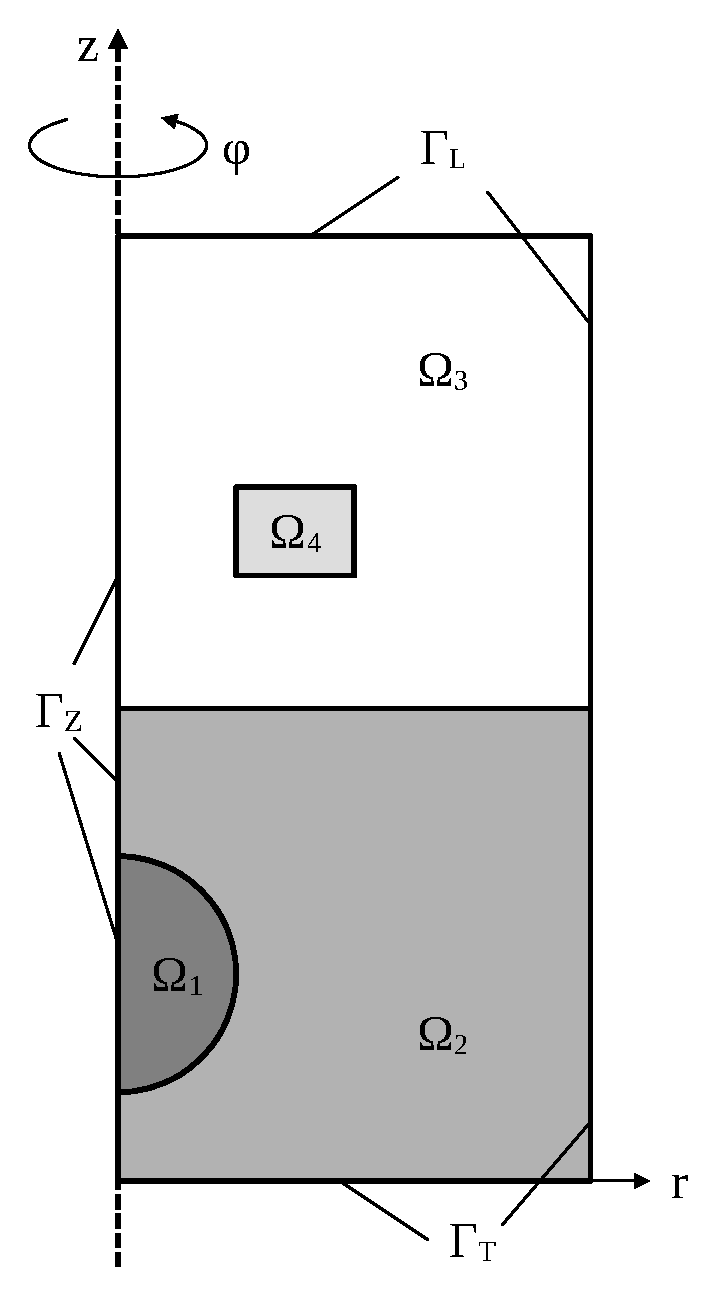
\includegraphics[width=0.9\linewidth]{elrendezes_2d.pdf}
        \caption{A szimulált elrendezés.}
        \label{fig:elrendezes_2d}
    \end{wrapfigure}

    \begin{align}
        \dfrac{\partial}{\partial \varphi} = 0
    \end{align}
    
    A tartományok jelentése: $\Omega_1$ -- vasgömb, $\Omega_2$ -- talaj, $\Omega_3$ -- levegő, $\Omega_4$ -- tekercs.

    Mivel csak egy adott $\omega$ körfrekvencián kell vizsgálódnunk, emiatt elég a szinuszos állandósult állapottal foglalkoznunk:
    \begin{align}
        \dfrac{\partial}{\partial t} \quad&\longrightarrow\quad j\omega
    \end{align}
    A kérdéses $\omega$ körfrekvencián az elektromágneses hullámok szabadtéri hullámhossza ($\varepsilon_r = 1$):
    \begin{align}
        \lambda &= \dfrac{c}{f} = \dfrac{c}{\dfrac{\omega}{2\pi}} = \dfrac{\qty{3e8}{\metre\per\second}}{\dfrac{2\pi\qty{500}{\per\second}}{2\pi}} = \qty{6e5}{\metre}
    \end{align}
    Emiatt $\lambda$ az \qty{1000}{km} nagyságrendjébe esik, míg az elrendezés fizikai méretei néhányszor \qty{10}{cm}-esek, így élhetünk a magneto-kvázistacionárius közelítéssel:
    \begin{align}
        \dfrac{\partial \vec{D}}{\partial t} \quad&\longrightarrow\quad 0
    \end{align}
    \clearpage
    Ebben az esetben a vizsgált tartományon belül a Maxwell-egyenleteknek a következő alakja érvényes:
    \begin{align}
        \rot \vec{H} &= \vec{J} \\
        \rot \vec{E} &= -j\omega\vec{B}\\
        \divergence \vec{B} &= 0\\
        \vec{B} &= \mu\vec{H}\\
        \vec{J} &= \sigma \vec{E} + \vec{J}_i
    \end{align}

    \begin{align}
        \sigma(\vec{r}) &=
            \begin{cases}
                \sigma, & \text{ha } \vec{r} \in \Omega_1\\
                \sigma_t, & \text{ha } \vec{r} \in \Omega_2\\
                0, & \text{ha } \vec{r} \in \Omega_3 \cup \Omega_4
            \end{cases}
    \end{align}

    Az $R$ sugarat megfelelően nagyra kell választani ahhoz, hogy a kialakuló teret ne befolyásolja jelentősen a vizsgált $\Omega$ tartomány $\Gamma_T \cup \Gamma_L$ ,,távoli'' peremének a közelsége.
    

    A feladat megoldásához az $\vec{A}-\Phi, \vec{A}$ formalizmust használjuk, mert az előadáson bemutatott indukciós főzőlapos példa alapján ezzel a megközelítéssel egy jól kezelhető parciális differenciálegyenlet-rendszert kapunk, amit a PDEtool segítségével megoldhatunk.
\begin{align}
    \vec{B} = \rot \vec{A}
\end{align}
A peremfeltételekről a következőket lehet tudni:
\begin{align}
    B_n(\vec{r}) &= 0, \quad \vec{r} \in \Gamma_Z\\
    B_n(\vec{r}) &= 0, \quad \vec{r} \in \Gamma_L \cup \Gamma_T
\end{align}
A $B_n$ normális mágneses indukció a $\Gamma_Z$ peremen a szimmetria miatt lesz 0, a $\Gamma_L \cup \Gamma_T$ távoli peremeken pedig a nagy távolság miatt lesz közel 0, amit pontosan 0 értékkel modellezünk.
\section{A PDE és megadása pdetool-ban}
A tartományokra vonatkozó parciális differenciálegyenlet:
\begin{equation}
    -\left(\dfrac{\partial}{\partial r}\dfrac{1}{r\mu}\dfrac{\partial(rA_{\varphi})}{\partial r}+\dfrac{\partial}{\partial z}\dfrac{1}{r\mu}\dfrac{\partial(rA_{\varphi})}{\partial z}\right) + j\omega\sigma A_{\varphi} = J_{i,\varphi}
\end{equation}
Ezt a következő helyettesítésekkel lehet MATLAB-ban (pdetool-ban) megadni:
\begin{equation}
    \begin{aligned}
        rA_{\varphi}\quad\rightarrow&\quad\verb|u|\\
        r\quad\rightarrow&\quad\verb|x|\\
        z\quad\rightarrow&\quad\verb|y|
    \end{aligned}
\end{equation}
A használt elliptikus PDE séma a következő:
\begin{equation}
    \verb|-div(c*grad(u))+a*u=f|
\end{equation}
Eszerint az egyes paraméterek behelyettesítési értékei:
\begin{equation}
    \begin{aligned}
        \verb|c|\quad=&\quad\dfrac{1}{r\mu}\\
        \verb|a|\quad=&\quad\dfrac{j\omega\sigma}{r}\\
        \verb|f|\quad=&\quad J_{i,\varphi}
    \end{aligned}
\end{equation}

    \section{Bak Bálint szekciója}
    dolgok

    \section{Impedancia kiszámítása $rA_{\varphi}$ értékekből}
%
A fluxusból tudunk következtetni a tekercs impedanciájára. A tekercs fluxusát
egyszerűen ki lehet számolni a PDE megoldásának eredményeként kapott háromszögekből.\\
%
Egy menetre számított fluxus számítása:
%
\begin{align}
    \Psi \triangleq \int_{s}^{}  \vec{B} \,ds
    \rightarrow  \Psi = \int_{s} rot(\vec{A}) \,ds
    = \oint_L \vec{A} \,dl
\end{align}
%
Ebből már meg tudjuk határozni, hogy a teljes tekercs fluxusát, amihez tudni kell még a
tekercs menetszámát(N) és a tekercs keresztmetsztét (F) amit a feladat meg adott.
%
Tekercs Fluxus számítása:
\begin{align}
    \Psi = \sum_{k = 1}^{N}  \Psi_k = \sum_{k = 1}^{N} \oint_{L_k} \vec{A} \,dl
    = \sum_{k = 1}^{N} 2 \pi r_k A_{\varphi,k}
\end{align}
%
A tekercs homogenizálásával számítható tekercs fluxus:
\begin{align}
    \Psi = \frac{1}{\Delta} \sum_{k=1}^N  2 \pi r_k A_{\varphi,k} \Delta F \approx
    \frac{N}{F} \int_{F} 2 \pi r_k A_{\varphi,k} \,dF
\end{align}
%
az integrál egyszerűen közelíthatő a FEM megoldásából, a háromszöghálóra felírt
integrál közelítő összeggel.
%
A kiszámított fluxusból már egyszrűen számítható a tekercs impedanciája is.
%
Kapocsfeszültség:
\begin{align}
    U = jw\Psi
\end{align}
Tekercs árama:
\begin{align}
    I = J_{\varphi} * \frac{F}{N}
\end{align}
Impedancia:
\begin{align}
    Z = \frac{U}{I} = \frac{jw\Psi}{I}
\end{align}
%
\section{A gömb méretének és mélységének változtatása}
%
\subsection{A földet tekintsük szigetelőnek}
%
\begin{align}
    \sigma_t\quad=\quad\qty{0}{\siemens\per\metre}
\end{align}
A pdetool-ban megadott PDE összetevők:\\
\vspace{0.2cm}
\begin{center}
\begin{tabular}{|l||c|c|c|}
    \hline
                    & \verb|c|                 & \verb|a|                   & \verb|f| \\
    \hline
    \hline
    Tekercs      & \verb|1./(4*pi*1e-7)./x| & \verb|0|                   & \verb|2000/(0.05*0.02)| \\
    \hline
    Levegő       & \verb|1./(4*pi*1e-7)./x| & \verb|0|                   & \verb|0| \\
    \hline
    Gömb         & \verb|1./(4*pi*1e-7)./x| & \verb|0|                   & \verb|0| \\
    \hline
    Talaj        & \verb|1./(4*pi*1e-7)./x| & \verb|j*2*pi*500*35e6./x|  & \verb|0| \\
    \hline
\end{tabular}\\
\end{center}
\vspace{0.5cm}
A peremeken mindenhol az \verb|1*u=0| Dirichlet-peremfeltételt adtuk meg. Ez egyben $A_{\varphi}$-re is Dirichlet-peremfeltételt jelent, ami miatt a peremeken $B_n=0$.\\[3ex]
%
Tekercs impedanciája gömb nélkül:
\begin{align}
    Z_0\quad=\quad0 + 1.2157\times10^3j\quad\Omega
\end{align}
%
A szimulációhoz konvergenciavizsgálatot végeztünk, aminél megvizsgáltuk a ritkább háló és a közelibb peremek hatását. A fenti alap esetben a hálót háromszor finomítottuk, illetve a szimulációs tartomány méretparamétere (a bal és jobb oldali perem távolsága) $R=\qty{0.5}{\metre}$ volt. Megvizsgáltuk az alap elrendezést szigetelő talajjal és gömb nélkül, de csak kétszeri hálófinomítás mellett. Így a tekercs impedanciájára a következő adódott:
\begin{align}
    Z_{0,mesh}\quad=&\quad0 + 1.2185\times10^3j\quad\Omega\\
    \dfrac{|Z_{0,mesh}-Z_0|}{|Z_0|}\quad=&\quad0.0023
\end{align}
%
Ezután megvizsgáltuk ugyanazt a kiinduló elrendezést, csak $R=\qty{0.3}{\metre}$ választással. Erre a következő tekercs induktivitás adódott:
\begin{align}
    Z_{0,R}\quad=&\quad0 + 1.2099\times10^3j\quad\Omega\\
    \dfrac{|Z_{0,R}-Z_0|}{|Z_0|}\quad=&\quad0.0048
\end{align}
%
Mindkét relatív hiba $1\%$ alatti, így elfogadhatjuk a részletesebb modellből kapott eredményeket, tehát innentől $R=0.5$ és háromszori hálófinomítást használunk.\\[3ex]
A tekercs impedanciája gömbbel, különböző paraméterekkel $[\Omega]$:
\vspace{0.2cm}
\begin{center}
\begin{tabular}{|c|c|c|c|}
    \hline
    \diagbox{r[m]}{d[m]} & 0.08                     & 0.13                     & 0.18                     \\
    \hline
    \hline
    0.01                 &                          & 5.4765e-03 + 1.2154e+03j &                          \\
    \hline
    0.03                 & 6.7525e-01 + 1.2124e+03j & 8.5124e-02 + 1.2153e+03j & 1.5855e-02 + 1.2156e+03j \\
    \hline
    0.05                 &                          & 3.5212e-01 + 1.2133e+03j &                          \\
    \hline
\end{tabular}\\
\end{center}
\vspace{0.5cm}
%
Innen tehát az impedancia megváltozása ($\Delta Z$) a gömb nálküli esethez képest [$\Omega$]:
\begin{center}
\begin{tabular}{|c|c|c|c|}
    \hline
    \diagbox{r[m]}{d[m]} & 0.08                     & 0.13                     & 0.18                     \\
    \hline
    \hline
    0.01                 &                          & 0.0055 - 0.3430j &                          \\
    \hline
    0.03                 & 0.6753 - 3.3430j & 0.0851 - 0.4430j & 0.0159 - 0.1430i \\
    \hline
    0.05                 &                          & 0.3521 - 2.4430i &                          \\
    \hline
\end{tabular}\\
\end{center}
\vspace{0.5cm}
%
A távolság csökentésével illetve a gömb átmérő csökkentésével csökken az impedancia reális
része míg a komplex szinte változatlan marad. Azaz a tekercsnek a gömb megjelenésével
lessz ellenállása is. Az ellenállás  nagysága pedig attól függ, hogy milyen távol van a gömb
a tekercstől és a gömb méretétől.
%
\subsection{A földet tekintsük rossz vezetőnek}
\begin{align}
    \sigma_t\quad=\quad\qty{1}{\siemens\per\metre}
\end{align}
A pdetool-ban megadott PDE összetevők:\\
\vspace{0.2cm}
\begin{center}
\begin{tabular}{|l||c|c|c|}
    \hline
                    & \verb|c|                 & \verb|a|                   & \verb|f| \\
    \hline
    \hline
    Tekercs      & \verb|1./(4*pi*1e-7)./x| & \verb|0|                   & \verb|1/(0.05*0.02)| \\
    \hline
    Levegő       & \verb|1./(4*pi*1e-7)./x| & \verb|0|                   & \verb|0| \\
    \hline
    Gömb         & \verb|1./(4*pi*1e-7)./x| & \verb|j*2*pi*500./x*1|     & \verb|0| \\
    \hline
    Talaj        & \verb|1./(4*pi*1e-7)./x| & \verb|j*2*pi*500*35e6./x|  & \verb|0| \\
    \hline
\end{tabular}\\
\end{center}
\vspace{0.5cm}
A peremeken mindenhol az \verb|1*u=0| Dirichlet-peremfeltételt adtuk meg.\\[3ex]
%
A tekercs impedanciája gömb nélkül: % + 
\begin{align}
    Z_0\quad=\quad6.6340\times10^{-4} + 1.2157\times10^3j \quad\Omega
\end{align}
A tekercs impedanciája gömbbel, különböző paraméterekkel $[\Omega]$:
%
\vspace{0.2cm}
\begin{center}
\begin{tabular}{|c|c|c|c|}
    \hline
    \diagbox{r[m]}{d[m]} & 0.08                     & 0.13                     & 0.18                     \\
    \hline
    \hline
    0.01                 &                          & 6.1399e-03 + 1.2154e+03j &                          \\
    \hline
    0.03                 & 6.7587e-01 + 1.2124e+03j & 8.5774e-02 + 1.2153e+03j & 1.6515e-02 + 1.2156e+03j \\
    \hline
    0.05                 &                          & 3.5271e-01 + 1.2133e+03j &                          \\
    \hline
\end{tabular}\\
\end{center}
\vspace{0.5cm}
%
Innen tehát az impedancia megváltozása ($\Delta Z$) a gömb nálküli esethez képest [$\Omega$]:
\vspace{0.2cm}
\begin{center}
\begin{tabular}{|c|c|c|c|}
    \hline
    \diagbox{r[m]}{d[m]} & 0.08                     & 0.13                     & 0.18                     \\
    \hline
    \hline
    0.01                 &                          & 0.0055 - 0.3430j &                          \\
    \hline
    0.03                 & 0.6752 - 3.3430j & 0.0851 - 0.4430j & 0.0159 - 0.1430j \\
    \hline
    0.05                 &                          & 0.3520 - 2.4430j &                          \\
    \hline
\end{tabular}\\
\end{center}
\vspace{0.5cm}
%
A tapasztalat szinte ugyanaz, mint amikor a földet szigetelőnek tekintjük, azzal a különbséggel, hogy a már a gömb nélkül is van valós része az impedanciának. Ez azért logikus, mert a véges vezetőképességű talajban létrejövő örvényáramok miatti ohmos veszteség jelenik meg a tekercs impedanciájának valós részeként. 
\subsection{A földet tekintsük jó vezetőnek}
A talaj vezetőképességét a volframéval megegyezőnek választottuk, mert az körülbelül fele a gömbre vonatkozónak, ami pedig az alumíniuménak felel meg.
\begin{align}
    \sigma_t\quad=\quad\qty{1.82e7}{\siemens\per\metre}
\end{align}
A pdetool-ban megadott PDE összetevők:\\
\vspace{0.2cm}
\begin{center}
\begin{tabular}{|l||c|c|c|}
    \hline
                    & \verb|c|                 & \verb|a|                   & \verb|f| \\
    \hline
    \hline
    Tekercs      & \verb|1./(4*pi*1e-7)./x| & \verb|0|                   & \verb|1/(0.05*0.02)| \\
    \hline
    Levegő       & \verb|1./(4*pi*1e-7)./x| & \verb|0|                   & \verb|0| \\
    \hline
    Gömb         & \verb|1./(4*pi*1e-7)./x| & \verb|j*2*pi*500./x*1.82e7|     & \verb|0| \\
    \hline
    Talaj        & \verb|1./(4*pi*1e-7)./x| & \verb|j*2*pi*500*35e6./x|  & \verb|0| \\
    \hline
\end{tabular}\\
\end{center}
\vspace{0.5cm}
A peremeken mindenhol az \verb|1*u=0| Dirichlet-peremfeltételt adtuk meg.\\[3ex]
%
A tekercs impedanciája gömb nélkül: % + 
\begin{align}
    Z_0\quad=\quad1.3793\times10^{1} + 1.0905\times10^3j \quad\Omega
\end{align}
A tekercs impedanciája gömbbel, különböző paraméterekkel $[\Omega]$:
%
\vspace{0.2cm}
\begin{center}
\begin{tabular}{|c|c|c|c|}
    \hline
    \diagbox{r[m]}{d[m]} & 0.08                     & 0.13                     & 0.18                     \\
    \hline
    \hline
    0.01                 &                          & 1.3922e+01 + 1.0902e+03j &                          \\
    \hline
    0.03                 & 1.3925e+01 + 1.0900e+03j & 1.3953e+01 + 1.0903e+03j & 1.3872e+01 + 1.0904e+03j \\
    \hline
    0.05                 &                          & 1.4064e+01 + 1.0901e+03j &                          \\
    \hline
\end{tabular}\\
\end{center}
\vspace{0.5cm}
%
Innen tehát az impedancia megváltozása ($\Delta Z$) a gömb nálküli esethez képest [$\Omega$]:
\vspace{0.2cm}
\begin{center}
\begin{tabular}{|c|c|c|c|}
    \hline
    \diagbox{r[m]}{d[m]} & 0.08                     & 0.13                     & 0.18                     \\
    \hline
    \hline
    0.01                 &                          & 0.1292 - 0.2737i &                          \\
    \hline
    0.03                 & 0.1322 - 0.4737i & 0.1602 - 0.1737j & 0.0792 - 0.0737i \\
    \hline
    0.05                 &                          & 0.2712 - 0.3737j &                          \\
    \hline
\end{tabular}\\
\end{center}
\vspace{0.5cm}
%
Az eredményekből arra lehet következtetni, hogy ha elég jó vezetőképességű a talaj, akkor az eltemetett jobb vezetőképességű gömb miatti impedancia megváltozás kisebb, mint a szigetelő vagy rossz vezetőképességű talaj esetén. Ha a talaj rossz vezető, akkor a gömb hatására megjelenő veszteség felhasználható detekcióra egy nagy jósági tényezőjű rezgőkör jósági tényezőjének lerontására, ami detektálható. Ellenben jó vezető talajnál már a tekercs impedanciájának valós része a gömb nélkül is számottevő, így a detekció sokkal nehezebb.
    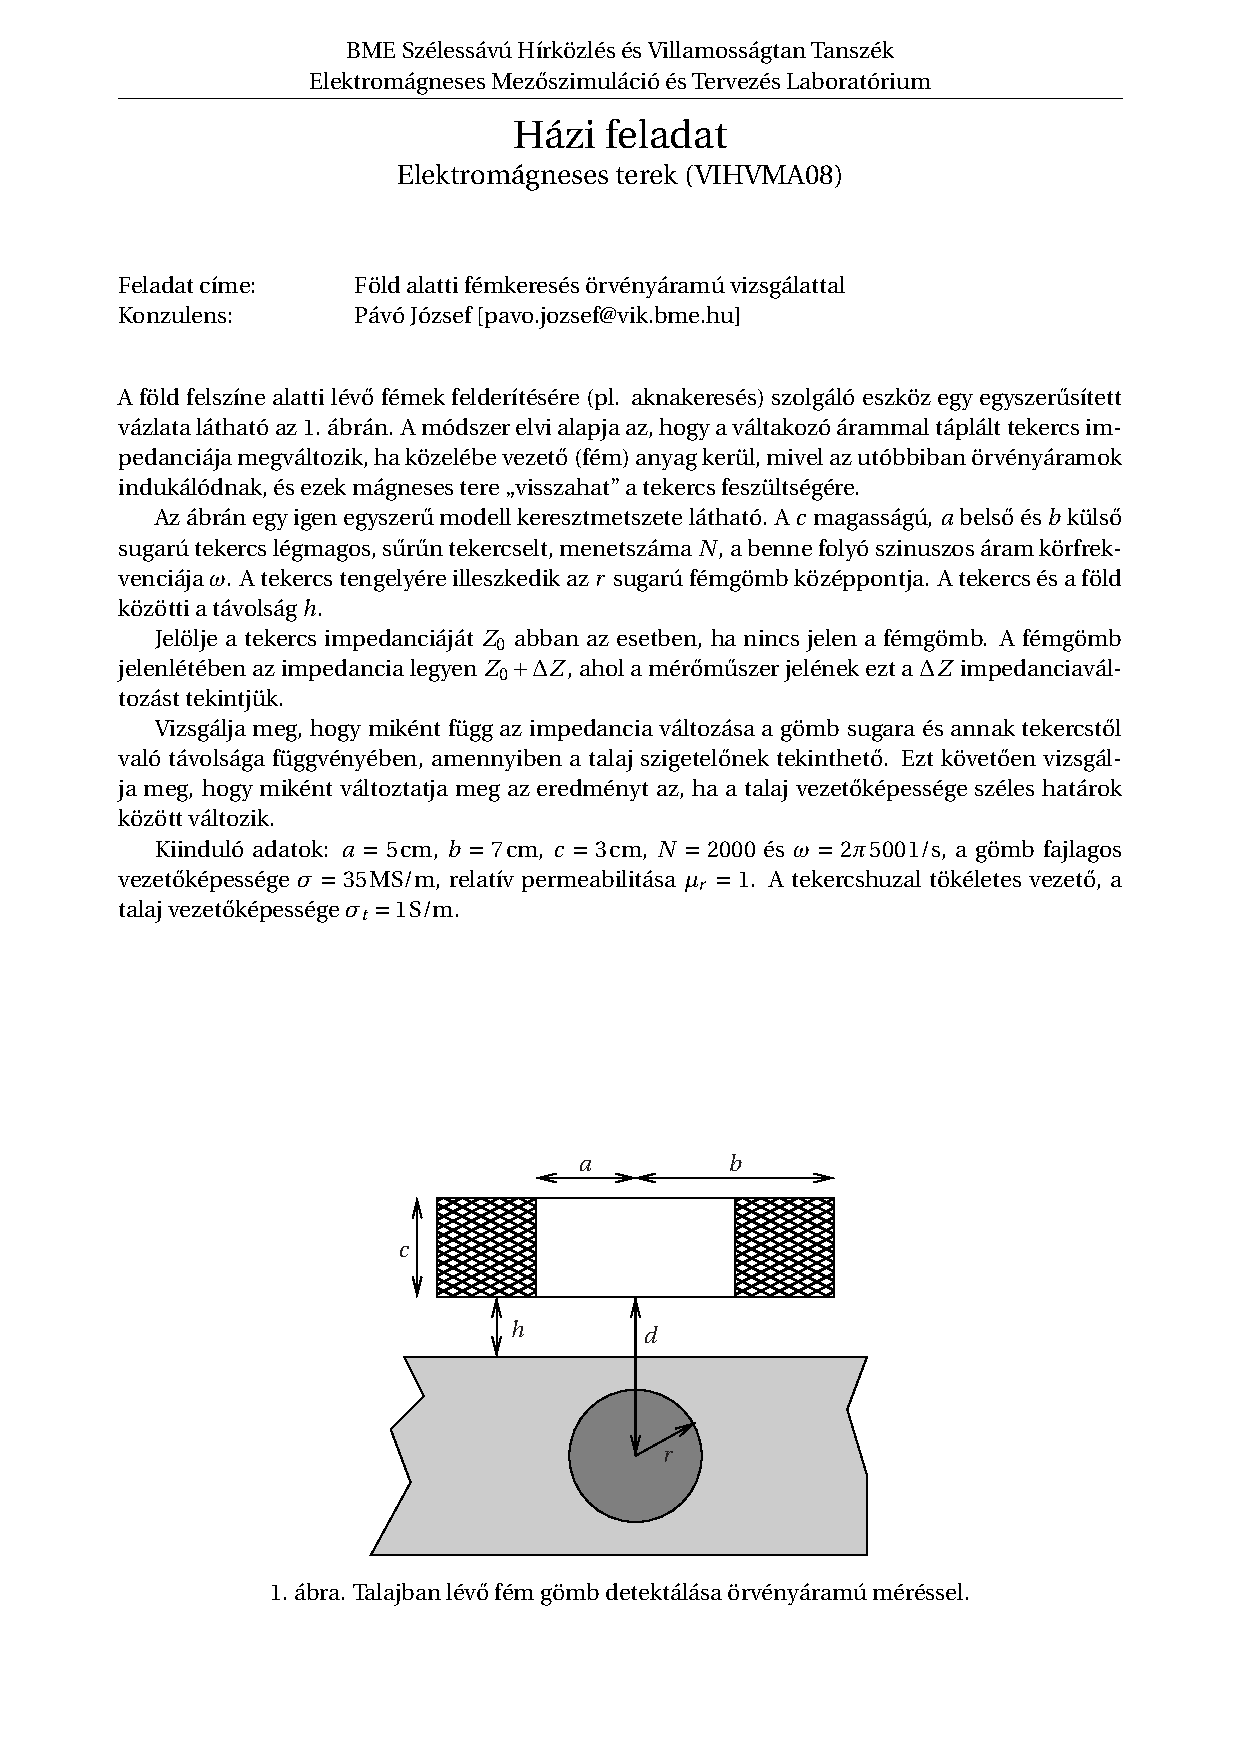
\includepdf{tartalom/feladatlap_femkereses.pdf}
%
\end{document}

%            \begin{figure}
%                \centering
%                \includegraphics[width=0.8\textwidth]{kep/szerkesztett/wstk-mighty-gecko-nagy.jpg}
%                \caption{WSTK + radio board.}
%                \label{fig:wstkmighty}
%            \end{figure}
% \cite{Anritsu}
%            \begin{figure}
%                \centering
%                \begin{subfigure}{0.48\textwidth}
%                    \includegraphics[width=\textwidth]{kep/szerkesztett/sol-868-conducted.png}
%                    \caption{\SI{868}{MHz}}
%                \end{subfigure}
%                \begin{subfigure}{0.48\textwidth}
%                    \includegraphics[width=\textwidth]{kep/szerkesztett/sol-470-conducted.png}
%                    \caption{\SI{470}{MHz}}
%                \end{subfigure}
%                \caption{470 és \SI{868}{MHz}-es Sol radio board-ok kimeneti spektruma.}
%                \label{fig:sol-conducted}
%            \end{figure}

